\documentclass[11pt,a4paper]{article}
\usepackage[utf8]{inputenc}
\usepackage[T1]{fontenc}
\usepackage[margin=2.4cm]{geometry}
\usepackage{amsmath,amssymb,amsthm,mathtools,bm}
\usepackage{booktabs,array,enumitem,xcolor}
\usepackage{tikz}
\usepackage{float}
\usetikzlibrary{arrows.meta,calc,positioning,decorations.pathreplacing,shapes.geometric,patterns}
\usepackage{pgfplots}
\pgfplotsset{compat=1.16}
\usepackage[most]{tcolorbox}
\usepackage[framemethod=tikz]{mdframed}
\usepackage[colorlinks=true,linkcolor=blue!50!black,urlcolor=blue!50!black]{hyperref}

% ---------- macros ----------
\newcommand{\E}{\mathbb{E}}
\newcommand{\R}{\mathbb{R}}
\newcommand{\tr}{\operatorname{tr}}
\newcommand{\argmin}{\operatorname*{arg\,min}}
\newcommand{\argmax}{\operatorname*{arg\,max}}
\newcommand{\Fx}{F_x}
\newcommand{\Fu}{F_u}
\newcommand{\Cx}{C_x}
\newcommand{\Cu}{C_u}
\newcommand{\slides}[1]{\emph{(slides #1)}}

% ---------- boxed amsthm environments ----------
\theoremstyle{plain}
\newmdtheoremenv[linecolor=black!70,linewidth=1pt,backgroundcolor=gray!6,innertopmargin=4pt,innerbottommargin=4pt]{theorem}{Theorem}[section]
\newmdtheoremenv[linecolor=black!70,linewidth=1pt,backgroundcolor=gray!6,innertopmargin=4pt,innerbottommargin=4pt]{proposition}[theorem]{Proposition}
\newmdtheoremenv[linecolor=black!70,linewidth=1pt,backgroundcolor=gray!6,innertopmargin=4pt,innerbottommargin=4pt]{lemma}[theorem]{Lemma}
\newmdtheoremenv[linecolor=black!70,linewidth=1pt,backgroundcolor=gray!6,innertopmargin=4pt,innerbottommargin=4pt]{corollary}[theorem]{Corollary}
\theoremstyle{definition}
\newmdtheoremenv[linecolor=green!40!black,linewidth=1pt,backgroundcolor=green!4,innertopmargin=4pt,innerbottommargin=4pt]{definition}[theorem]{Definition}
\newmdtheoremenv[linecolor=orange!70!black,linewidth=1pt,backgroundcolor=orange!5,innertopmargin=4pt,innerbottommargin=4pt]{algorithm}[theorem]{Algorithm}
\newmdtheoremenv[linecolor=purple!60!black,linewidth=1pt,backgroundcolor=purple!4,innertopmargin=4pt,innerbottommargin=4pt]{example}[theorem]{Example}
\theoremstyle{remark}
\newtheorem*{remark}{Remark}

% ---------- Intuition box ----------
\newtcolorbox{intuition}{enhanced,breakable,colback=blue!5,colframe=blue!60!black,
  coltitle=white,fonttitle=\bfseries,title={Intuition},boxrule=0.8pt,arc=2pt,
  left=6pt,right=6pt,top=4pt,bottom=4pt}

% ---------- placeholder for images to paste from the slides ----------
\newcommand{\slideplaceholder}[3]{%
  \begin{center}
  \begin{tikzpicture}
    \node[draw=red!60!black,dashed,very thick,fill=red!4,minimum width=#1,minimum height=#2,
          text width=#1-1cm,align=center,font=\small] {%
      \textbf{[Image to insert]}\\[2pt] #3};
  \end{tikzpicture}
  \end{center}}

\title{\textbf{Lecture 06 --- LQR, iLQR, MPC}\\[4pt]
\large Reinforcement Learning 2026--27 \\ Lecture notes based on the slide deck (slides 1--93) and the companion notes ``Finite-horizon MDPs and optimal control'' and ``LQR, iLQR, MPC''}
\author{}
\date{}

\begin{document}
\maketitle
\vspace{-1.5cm}
\begin{abstract}\noindent
These notes follow the \emph{order of the slides}: each section/subsection carries the (near-verbatim) slide title and, in parentheses, the slide range. The formal statements and proofs of the two companion PDFs are merged at the point where the slides introduce the topic. After each formal result there is a blue \emph{Intuition} box. Material that appears only in the PDFs and has no slide is collected in Appendix~\ref{app:supp}. Where a figure of the slides could not be redrawn (animated GIFs), a red dashed placeholder says which image to paste and where it comes from.
\end{abstract}
\tableofcontents
\newpage

%=====================================================================
\section{Recap \slides{2--10}}
%=====================================================================

The deck opens with a recap of the dynamic-programming algorithms for (infinite-horizon, discounted) MDPs, to set the stage for the control setting.

\subsection{Policy Iteration \slides{3--6}}

Policy iteration outputs a \emph{policy} at every iteration, $\{\pi_0,\pi_1,\pi_2,\dots,\pi_T\}$, whereas value iteration outputs \emph{values}. The procedure is:
\begin{enumerate}[nosep]
  \item start with a random guess $\pi_0$ (deterministic or stochastic);
  \item for $t=0,\dots,T$: do \emph{policy evaluation}, i.e.\ compute $Q^{\pi_t}(s,a)$ for all $(s,a)$; then \emph{policy improvement}, $\pi_{t+1}(s)\in\arg\max_a Q^{\pi_t}(s,a)$.
\end{enumerate}
The algorithm only makes progress: the performance of the policy is monotonically non-decreasing.

\begin{figure}[H]
\centering
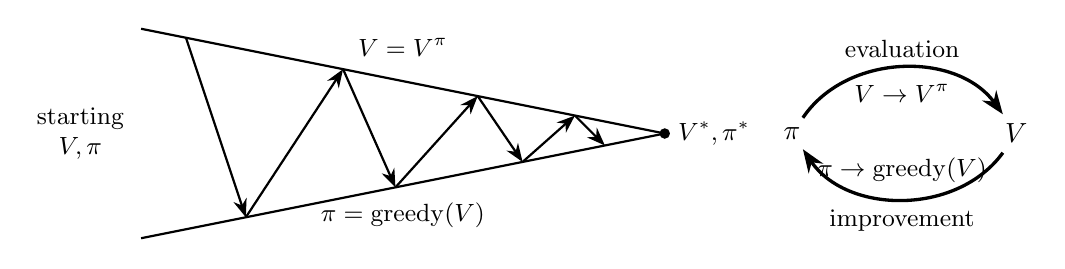
\begin{tikzpicture}[scale=0.95,>=Stealth]
  % left: zig-zag between V = V^pi and pi = greedy(V)
  \draw[thick] (0,2.4) -- (7,1);
  \draw[thick] (0,-0.4) -- (7,1);
  \node[above,sloped] at (3.5,1.9) {\small $V=V^{\pi}$};
  \node[below,sloped] at (3.5,0.2) {\small $\pi=\mathrm{greedy}(V)$};
  \node[left,align=center] at (-0.1,1.0) {\small starting\\[-1pt]\small $V,\pi$};
  \coordinate (a) at (0.6,2.28);
  \coordinate (b) at (1.4,-0.12);
  \coordinate (c) at (2.7,1.86);
  \coordinate (d) at (3.4,0.28);
  \coordinate (e) at (4.5,1.5);
  \coordinate (f) at (5.1,0.62);
  \coordinate (g) at (5.8,1.24);
  \coordinate (h) at (6.2,0.84);
  \draw[->,thick] (a)--(b); \draw[->,thick] (b)--(c); \draw[->,thick] (c)--(d);
  \draw[->,thick] (d)--(e); \draw[->,thick] (e)--(f); \draw[->,thick] (f)--(g);
  \draw[->,thick] (g)--(h);
  \fill (7,1) circle (2pt); \node[right] at (7.05,1) {\small $V^*,\pi^*$};
  % right: evaluation / improvement cycle
  \begin{scope}[xshift=10.2cm,yshift=1cm]
    \node (p) at (-1.5,0) {$\pi$}; \node (v) at (1.5,0) {$V$};
    \draw[->,very thick] (p) to[bend left=55] node[above] {\small evaluation} node[below=2pt] {\small $V\to V^{\pi}$} (v);
    \draw[->,very thick] (v) to[bend left=55] node[below] {\small improvement} node[above=2pt] {\small $\pi\to\mathrm{greedy}(V)$} (p);
  \end{scope}
\end{tikzpicture}
\caption{Redrawn from slide~4 (credits on the slide: David Silver). Left: policy iteration alternates two projections and spirals into $(V^*,\pi^*)$. Right: the evaluation/improvement cycle.}
\end{figure}

\paragraph{Properties (slides 5--6).} Is there a maximum number of iterations? Yes: $|A|^{|S|}$, the number of deterministic policies. Since each improvement step is monotone, a policy can appear in at most one round unless it is already optimal. \emph{Stopping rule:} stop when the policy does not change any more in any state.

\begin{intuition}
Policy iteration is a ``coordinate ascent'' between two objects: given a policy, you can compute exactly how good it is (evaluation); given values, you can read off a policy that is at least as good (greedy improvement). Because each round can only help, and there are finitely many policies, you cannot cycle: you must land on the optimum.
\end{intuition}

\subsection{We Did Dynamic Programming! \slides{7--8}}

Dynamic programming applies when there is (i) \textbf{optimal substructure} (the optimal solution decomposes into subproblems) and (ii) \textbf{overlapping subproblems} (subproblems recur and their solutions can be cached). MDPs have both, thanks to the Bellman equation. We used DP for \emph{planning}: we assumed the transition probabilities of the MDP are known.

\begin{table}[h]
\centering
\begin{tabular}{@{}lll@{}}
\toprule
\textbf{Problem} & \textbf{Bellman equation} & \textbf{Algorithm}\\
\midrule
Prediction & Bellman expectation equation & Iterative policy evaluation\\
Control & Bellman expectation eq.\ + greedy improvement & Policy iteration\\
Control & Bellman optimality equation & Value iteration\\
\bottomrule
\end{tabular}
\caption{Table of slide~8 (credits: David Silver), retyped.}
\end{table}

\subsection{Primal Linear Program \slides{9}}

As an alternative to VI and PI, the Bellman optimality equation can be written as a linear program: minimise $\sum_s V(s)$ subject to the Bellman inequalities $V(s)\ge r(s,a)+\gamma\sum_{s'}p(s'\mid s,a)V(s')$ for all $(s,a)$. The optimal $V^*$ is the pointwise smallest feasible vector, hence the unique minimiser. (The slide shows the objective ``$\min V(s)$'' and the constraints as images; this is the standard form.)

\begin{intuition}
Any $V$ that satisfies all Bellman inequalities is an \emph{upper bound} on what any policy can achieve; the best upper bound that is still valid is $V^*$ itself. A linear program finds it without iterating Bellman updates.
\end{intuition}

%=====================================================================
\section{Finite-Horizon MDPs \slides{11--25}}
%=====================================================================

\subsection{Definition and time-dependent policies \slides{11--15}}

The deck uses a slightly different formulation: $(S,A,R,T,H,\mu_0)$, with horizon $H$ and initial-state distribution $s_0\sim\mu_0$. (The companion notes write the same object as $(S,A,p,r,H,\mu)$, $H\ge 1$.)

\begin{definition}[Finite-horizon MDP]\label{def:fhmdp}
A finite-horizon MDP is a tuple $(S,A,p,r,H,\mu)$ with horizon $H\ge1$ and initial distribution $s_0\sim\mu$. An \emph{episode} is $s_0,a_0,s_1,\dots,s_{H-1},a_{H-1}$, and there is \emph{no discount factor}. Policies are \emph{time-dependent}: $\pi=(\pi_0,\pi_1,\dots,\pi_{H-1})$ with $a_h=\pi_h(s_h)$.
\end{definition}

The slides stress (slides 13--15): the action may differ for the same state depending on $t$ (e.g.\ ``I could explore more at the beginning''), and this is \emph{very common in control}.

\begin{intuition}
With a deadline, the \emph{time remaining} is part of the situation. Think of an exam: with two hours left you explore a hard problem; with two minutes left you write down what you have. The same state (``this question is open'') calls for different actions. A stationary policy cannot express that; a time-dependent one can. A concrete numerical example where this is \emph{necessary} is in Appendix~\ref{app:supp}.
\end{intuition}

\subsection{Finite-Horizon MDPs --- Example \slides{16}}

The slide shows a wheeled robot that must follow a reference trajectory: state $(X(t),Y(t))$ (plus orientation), controls $v$ (forward speed) and $\omega$ (turn rate), reference point $(X_r(t),Y_r(t))$. The cost penalises the distance to the moving reference over a finite horizon, which is a natural finite-horizon problem.

\begin{figure}[H]
\centering
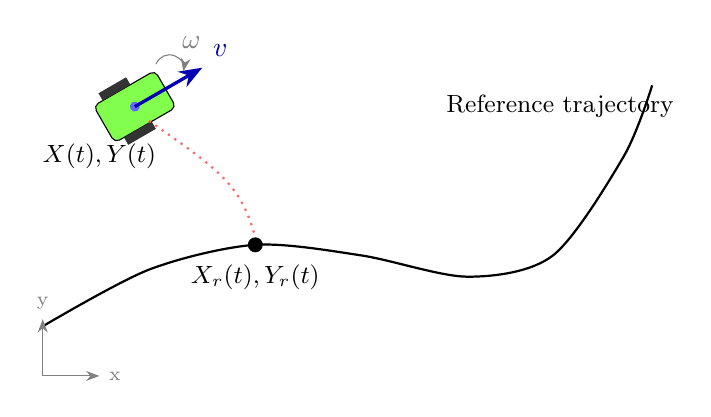
\begin{tikzpicture}[>=Stealth,scale=0.9]
  \draw[thick,smooth] plot coordinates {(0,0.2)(1.5,1)(3,1.35)(4.5,1.2)(6,0.9)(7.2,1.2)(8.2,2.6)(8.6,3.6)};
  \node at (7.3,3.3) {\small Reference trajectory};
  \fill (3,1.35) circle (3pt);
  \node[below] at (3,1.2) {\small $X_r(t),Y_r(t)$};
  \begin{scope}[shift={(1.3,3.3)},rotate=30]
    \draw[fill=green!60!lime!70,rounded corners=2pt] (-0.5,-0.3) rectangle (0.5,0.3);
    \fill[black!80] (-0.35,-0.42) rectangle (0.1,-0.3);
    \fill[black!80] (-0.35,0.3) rectangle (0.1,0.42);
    \fill[blue!60] (0,0) circle (2pt);
    \draw[->,blue!70!black,very thick] (0,0) -- (1.1,0) node[above right] {$v$};
  \end{scope}
  \draw[->,gray] (1.6,3.9) arc (160:-10:0.2);
  \node[gray] at (2.1,4.2) {$\omega$};
  \node at (0.8,2.6) {\small $X(t),Y(t)$};
  \draw[red!60,dotted,thick] (1.5,3.1) .. controls (2.5,2.4) and (2.8,2.2) .. (3,1.45);
  \draw[->,gray] (0,-0.5)--(0,0.3) node[above] {\scriptsize y};
  \draw[->,gray] (0,-0.5)--(0.8,-0.5) node[right] {\scriptsize x};
\end{tikzpicture}
\caption{Redrawn from the example on slide~16: a robot with state $(X,Y)$ and controls $(v,\omega)$ tracking a moving reference point.}
\end{figure}

\subsection{Finite-Horizon MDP \& Policy Interaction \slides{17--21}}

The slides build the interaction step by step: $s_0\sim\mu_0$; the policy picks $a_0$; the environment draws $s_1\sim P(\cdot\mid s_0,a_0)$; the policy picks $a_1$; \dots; until the episode $(s_0,a_0,s_1,a_1,\dots,s_{H-1},a_{H-1})$ is complete.

\begin{center}
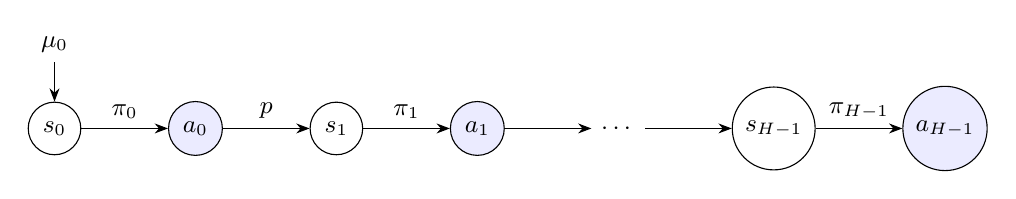
\begin{tikzpicture}[>=Stealth,node distance=1.1cm,every node/.style={font=\small}]
  \node[circle,draw] (s0) {$s_0$};
  \node[circle,draw,right=of s0,fill=blue!8] (a0) {$a_0$};
  \node[circle,draw,right=of a0] (s1) {$s_1$};
  \node[circle,draw,right=of s1,fill=blue!8] (a1) {$a_1$};
  \node[right=of a1] (dots) {$\cdots$};
  \node[circle,draw,right=of dots] (sH) {$s_{H-1}$};
  \node[circle,draw,right=of sH,fill=blue!8] (aH) {$a_{H-1}$};
  \draw[->] (s0)--node[above]{$\pi_0$}(a0);
  \draw[->] (a0)--node[above]{$p$}(s1);
  \draw[->] (s1)--node[above]{$\pi_1$}(a1);
  \draw[->] (a1)--(dots);
  \draw[->] (dots)--(sH);
  \draw[->] (sH)--node[above]{$\pi_{H-1}$}(aH);
  \node[above=0.5cm of s0] (m) {$\mu_0$}; \draw[->] (m)--(s0);
\end{tikzpicture}
\end{center}

\subsection{Finite-Horizon MDP: $V$ \& $Q$ \slides{22--24}}

With no discount factor, for $s_h=s$, $a_\tau=\pi_\tau(s_\tau)$ and $s_{\tau+1}\sim P(\cdot\mid s_\tau,a_\tau)$:
\[
V^\pi_h(s)=\E_\pi\Big[\sum_{\tau=h}^{H-1} r(s_\tau,a_\tau)\Big],\qquad
Q^\pi_h(s,a)=r(s,a)+\E_{s'\sim p(\cdot\mid s,a)}\big[V^\pi_{h+1}(s')\big],
\]
where in $Q^\pi_h$ the first action is $a_h=a$ and afterwards $\pi$ is followed. The optimal policy is the collection $\pi^*=\{\pi^*_0,\pi^*_1,\dots,\pi^*_{H-1}\}$ (slide 26).

\subsection{Finite-Horizon MDP: Bellman Equation \slides{25}}

The Bellman equation links consecutive levels: $V^\pi_h(s)=Q^\pi_h(s,\pi_h(s))$ and $Q^\pi_h(s,a)=r(s,a)+\E_{s'}[V^\pi_{h+1}(s')]$, i.e.\ level $h$ depends on level $h+1$ \emph{only}.

\begin{intuition}
$V_h$ is the ``reward-to-go'' with $H-h$ steps left. The Bellman equation says: reward-to-go = reward now + average reward-to-go from wherever you land. Level $h+1$ has already been paid for, so you only have to think one step ahead. This is precisely the structure that lets you compute everything by \emph{walking backwards from the deadline}.
\end{intuition}

%=====================================================================
\section{Finding the Optimal Policy \slides{26--32}}
%=====================================================================

The slides note: this is an \emph{easier problem than the infinite-horizon one}. We reason backwards in time and apply dynamic programming. At the last step $H-1$ there is no future, so $Q^*_{H-1}(s,a)=r(s,a)$; then we ask what happens at $H-2$, and so on (slides 27--32).

\begin{algorithm}[Backward induction / finite-horizon value iteration]\label{alg:bi}
\begin{enumerate}[nosep]
  \item At the last step: $Q^*_{H-1}(s,a)=r(s,a)$, $\ \pi^*_{H-1}(s)\in\arg\max_a Q^*_{H-1}(s,a)$, $\ V^*_{H-1}(s)=\max_a Q^*_{H-1}(s,a)$.
  \item For $h=H-2,H-3,\dots,0$:
  \begin{align*}
  Q^*_h(s,a)&=r(s,a)+\E_{s'\sim p(\cdot\mid s,a)}\big[V^*_{h+1}(s')\big],\\
  \pi^*_h(s)&\in\arg\max_a Q^*_h(s,a),\qquad V^*_h(s)=\max_a Q^*_h(s,a).
  \end{align*}
\end{enumerate}
\end{algorithm}

\begin{theorem}[Backward induction is exact (SKIPPED IN CLASS)]\label{thm:bi}
Algorithm~\ref{alg:bi} returns $V^*_h=\max_\pi V^\pi_h$ for every $h$ and every state, and $\pi^*=(\pi^*_0,\dots,\pi^*_{H-1})$ is optimal. The cost is $O(H|S|^2|A|)$ and there is no approximation error at any step.
\end{theorem}
\begin{proof}
Backward induction on $h$. At $h=H-1$ no future remains, so $V^\pi_{H-1}(s)=r(s,\pi_{H-1}(s))$ for any $\pi$, and taking the maximum over $a$ is optimal by inspection; the maximum is attained because $A$ is finite.

Suppose $V^*_{h+1}$ is the optimal value at level $h+1$. For any policy $\pi$, by the Bellman equation of the previous section,
\[
V^\pi_h(s)=r(s,\pi_h(s))+\E_{s'}[V^\pi_{h+1}(s')]\le r(s,\pi_h(s))+\E_{s'}[V^*_{h+1}(s')]\le\max_a\big[r(s,a)+\E_{s'}[V^*_{h+1}(s')]\big],
\]
the first inequality by the induction hypothesis and the second because the maximum dominates any particular action. The right-hand side is exactly $V^*_h(s)$ as computed by the algorithm, and it is attained by the policy that plays $\pi^*_h$ now and behaves optimally afterwards, which exists by the induction hypothesis. Hence $V^*_h$ is the optimal value and $\pi^*_h$ attains it.

\emph{Cost.} Each of the $H$ levels evaluates $|S||A|$ pairs, each requiring an expectation over $|S|$ successors.
\end{proof}

\begin{center}
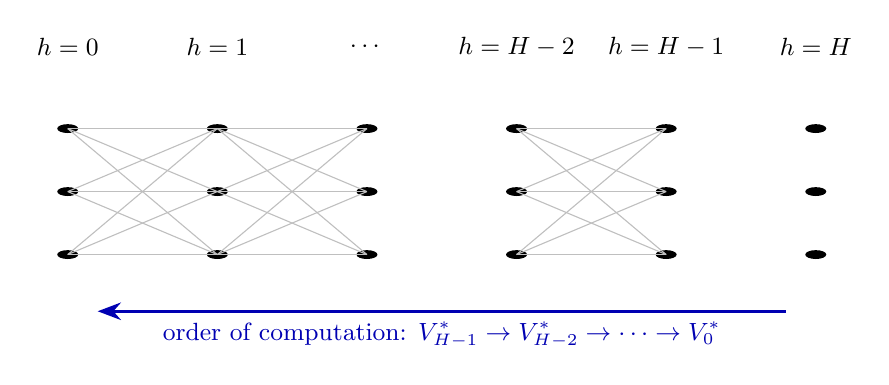
\begin{tikzpicture}[>=Stealth,xscale=1.9,yscale=0.8,every node/.style={font=\small}]
  \foreach \h/\lab in {0/{h=0},1/{h=1},2/{\cdots},3/{h=H-2},4/{h=H-1},5/{h=H}} {
    \node at (\h,3.3) {$\lab$};
    \foreach \s in {0,1,2} \fill (\h,\s) circle (2pt);
  }
  \foreach \h in {0,1,3} {
    \pgfmathtruncatemacro{\n}{\h+1}
    \foreach \s in {0,1,2} \foreach \t in {0,1,2} \draw[gray!50] (\h,\s)--(\n,\t);
  }
  \draw[->,very thick,blue!70!black] (4.8,-0.9)--(0.2,-0.9) node[midway,below] {order of computation: $V^*_{H-1}\to V^*_{H-2}\to\cdots\to V^*_0$};
\end{tikzpicture}
\end{center}

\begin{intuition}
It is like computing the cheapest route backwards from the destination. At the end there is nothing to plan: pick the best immediate reward. One step earlier, the only thing you need to know about the future is the value table you just built --- not the many futures that lead to it. Each stage costs one sweep, so the total is linear in the horizon, and nothing is approximated. That is why the finite-horizon problem is \emph{easier}: no fixed-point equation, just one pass.
\end{intuition}

%=====================================================================
\section{Control Problems and Optimal Control \slides{33--39}}
%=====================================================================

\subsection{Control Problems \slides{33--36}}

So far the state and action spaces were discrete. What about a cartpole? State: angular position \& velocity, linear position \& velocity; action/control: the force on the cart; goal: find the control policy that minimises the long-term cost. More generally in control $x\in\R^d$ and $u\in\R^k$; we write \textbf{$x$ for the state and $u$ for the action}, and we talk about \textbf{cost} rather than reward: we \emph{minimise} cost.

\begin{figure}[H]
\centering
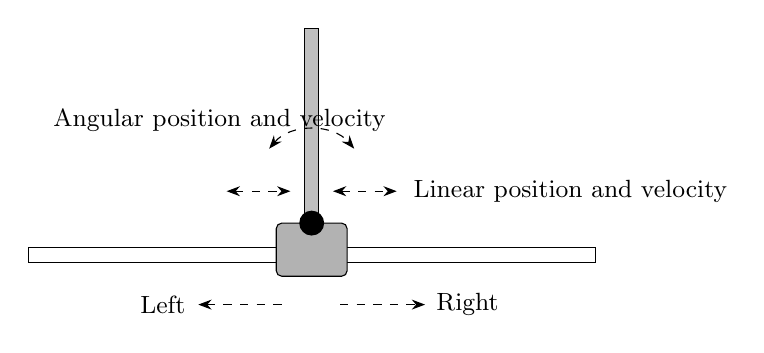
\begin{tikzpicture}[>=Stealth,scale=0.9,every node/.style={font=\small}]
  \draw[fill=white] (-4,-0.1) rectangle (4,0.1);
  \draw[fill=gray!60,rounded corners=2pt] (-0.5,-0.3) rectangle (0.5,0.45);
  \draw[fill=gray!50] (-0.1,0.4) rectangle (0.1,3.2);
  \fill (0,0.45) circle (5pt);
  \draw[<->,dashed] (-1.2,0.9) -- (-0.3,0.9) ;
  \draw[<->,dashed] (0.3,0.9) -- (1.2,0.9) ;
  \node[right] at (1.3,0.9) {Linear position and velocity};
  \draw[<->,dashed] (-0.6,1.5) to[bend left=50] (0.6,1.5);
  \node[above] at (-1.3,1.6) {Angular position and velocity};
  \draw[<-,dashed] (-1.6,-0.7)--(-0.4,-0.7); \node at (-2.1,-0.7) {Left};
  \draw[->,dashed] (0.4,-0.7)--(1.6,-0.7); \node at (2.2,-0.7) {Right};
\end{tikzpicture}
\caption{Cartpole, redrawn from slides 33--34: four state variables, one scalar control (horizontal force).}
\end{figure}

\subsection{Optimal Control \slides{37--39}}

\begin{definition}[Optimal control problem]
Given a dynamical system with non-linear transition function $f$, state $x\in\R^d$ and control $u\in\R^k$, find a control policy $\pi$ such that
\[
\min_\pi\ \E_\pi\Big[c_H(x_H)+\sum_{h=0}^{H-1}c_h(x_h,u_h)\Big],\qquad u_h=\pi(x_h),\ x_0\sim\mu_0 .
\]
\end{definition}

This looks very familiar: can we treat it as a finite-horizon MDP and use value iteration? \textbf{Approach 1: discretise.}

%=====================================================================
\section{Discretization and Bellman's Curse of Dimensionality \slides{40--42} (SKIPPED IN CLASS)}
%=====================================================================

Discretise each coordinate of $x\in\R^d$ and $u\in\R^k$ at resolution $\epsilon$. The number of grid points grows exponentially with the dimension (slide 40): $(1/\epsilon)^d$ states and $(1/\epsilon)^k$ actions. In practice discretisation is only computationally feasible up to \textbf{5 or 6 dimensional} state spaces (slides 41--42). \textbf{Approach 2:} work directly in continuous space, starting from simplified problems.

\begin{proposition}[Bellman's curse of dimensionality]\label{prop:curse}
Discretising each dimension of $x$ and $u$ at resolution $\epsilon$ gives $|S|=\Theta((1/\epsilon)^d)$ and $|A|=\Theta((1/\epsilon)^k)$, so one level of backward induction costs $\Theta((1/\epsilon)^{2d+k})$ operations with a dense transition table, and $\Theta((1/\epsilon)^{d+k})$ when the dynamics are deterministic and each state-action pair has a single successor cell.
\end{proposition}
\begin{proof}
A hypercube of side $1$ discretised at resolution $\epsilon$ has $1/\epsilon$ points per dimension. The sweep cost of Theorem~\ref{thm:bi} is $|S|^2|A|$ per level, because the expectation over $s'$ has $|S|$ terms; with a single successor it has one, and the cost is $|S||A|$.
\end{proof}

\begin{figure}[H]
\centering
\begin{minipage}{0.4\linewidth}
\centering
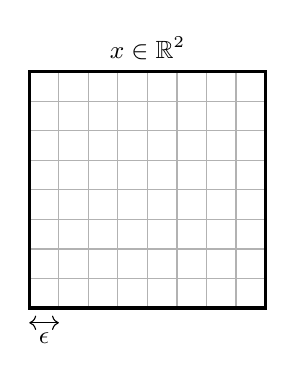
\begin{tikzpicture}[scale=0.75]
  \draw[step=0.5,gray!60] (0,0) grid (4,4);
  \draw[very thick] (0,0) rectangle (4,4);
  \draw[<->] (0,-0.25)--(0.5,-0.25) node[midway,below] {\small $\epsilon$};
  \node at (2,4.4) {\small $x\in\R^2$};
\end{tikzpicture}
\end{minipage}\hfill
\begin{minipage}{0.58\linewidth}
\centering
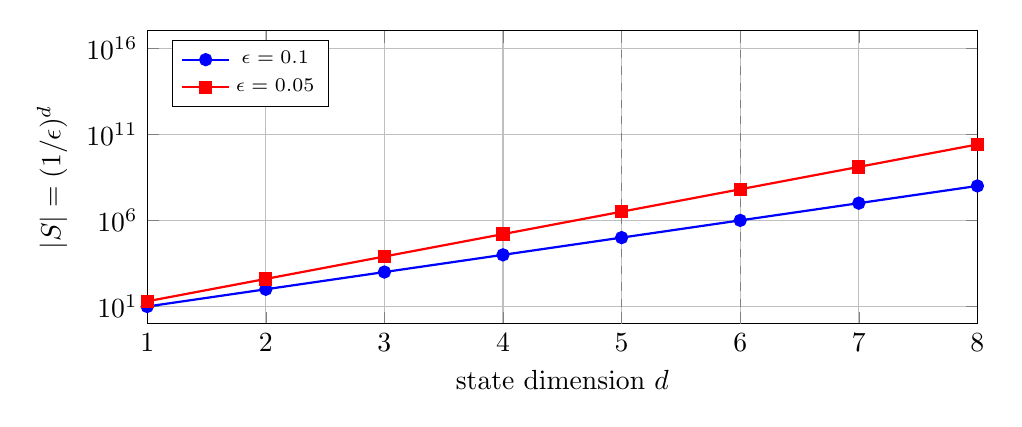
\begin{tikzpicture}
\begin{axis}[width=\linewidth,height=5.3cm,ymode=log,xlabel={state dimension $d$},ylabel={$|S|=(1/\epsilon)^d$},
  legend pos=north west,legend style={font=\scriptsize},grid=both,xmin=1,xmax=8,ymax=1e17,ymin=1]
\addplot[blue,thick,mark=*] coordinates {(1,10)(2,100)(3,1000)(4,1e4)(5,1e5)(6,1e6)(7,1e7)(8,1e8)};
\addlegendentry{$\epsilon=0.1$}
\addplot[red,thick,mark=square*] coordinates {(1,20)(2,400)(3,8000)(4,1.6e5)(5,3.2e6)(6,6.4e7)(7,1.28e9)(8,2.56e10)};
\addlegendentry{$\epsilon=0.05$}
\draw[dashed,gray] (axis cs:5,1) -- (axis cs:5,1e17);
\draw[dashed,gray] (axis cs:6,1) -- (axis cs:6,1e17);
\end{axis}
\end{tikzpicture}
\end{minipage}
\caption{Left: grid at resolution $\epsilon$ (slide 40). Right: original illustration of the exponential growth; the dashed lines mark the 5--6 dimensions that the slides give as the practical limit.}
\end{figure}

\begin{intuition}
Halving $\epsilon$ multiplies the number of cells by $2^d$. A 6-dimensional state at $\epsilon=0.05$ already has $6.4\times10^7$ cells, and with a dense transition table the sweep costs the \emph{square} of that times $|A|$. (The slide writes the grid size as a sum $(1/\epsilon)^d+(1/\epsilon)^k$; the number of state-action \emph{pairs} that the sweep must touch is the product $(1/\epsilon)^{d+k}$, which is what Proposition~\ref{prop:curse} counts.) Discretisation is not wrong --- it is just \emph{exponentially expensive}, which motivates looking for problems where the continuous solution has a closed form.
\end{intuition}

%=====================================================================
\section{Linear Systems and Quadratic Cost \slides{43--46}}
%=====================================================================

\subsection{Linear Systems \slides{43--44}}

Consider the system
\[
x_{t+1}=F_x x_t+F_u u_t,\qquad F_x\in\R^{d\times d},\ F_u\in\R^{d\times k},
\]
where $x_t$ is the state and $u_t$ the control (action) at time $t$. This \emph{is} our transition function.

\subsection{Quadratic Cost Function \slides{45--46}}

\begin{definition}[Linear-quadratic regulator (LQR)]\label{def:lqr}
$x_{t+1}=F_xx_t+F_uu_t$, $\ c(x,u)=x^\top C_xx+u^\top C_uu$, with $C_x\succeq0$ symmetric and $C_u\succ0$ symmetric. The problem is to minimise $\E\big[x_H^\top C_xx_H+\sum_{h=0}^{H-1}c(x_h,u_h)\big]$.
\end{definition}

(The slides ask for $C_x,C_u$ both positive definite, so that any non-zero state costs something even with all-zero control; the companion notes only require $C_x\succeq0$, which is what the proof needs.) The slides also use the alternative notation $g(x_t,u_t)$ for the cost.

\begin{figure}[H]
\centering
\begin{minipage}{0.48\linewidth}
\centering
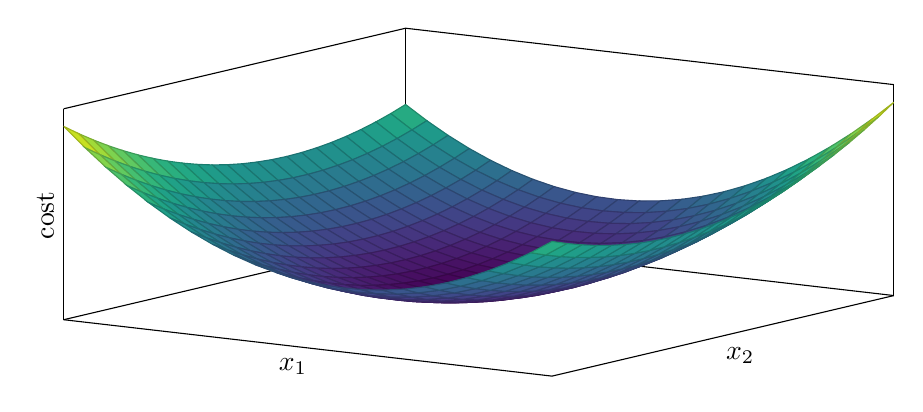
\begin{tikzpicture}
\begin{axis}[width=\linewidth,height=6cm,view={35}{25},xlabel={$x_1$},ylabel={$x_2$},zlabel={cost},ticks=none,colormap/viridis,
  xmin=-1,xmax=1,ymin=-1,ymax=1]
\addplot3[surf,domain=-1:1,y domain=-1:1,samples=24,samples y=24] {x^2+0.5*y^2+0.3*x*y};
\end{axis}
\end{tikzpicture}
\end{minipage}\hfill
\begin{minipage}{0.48\linewidth}
\centering
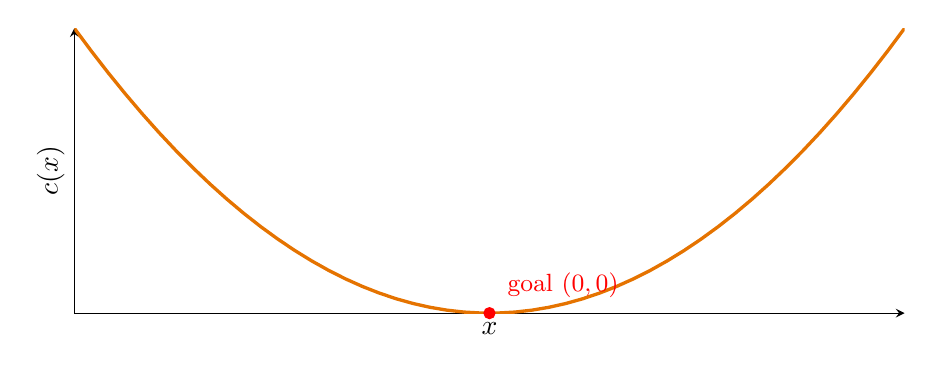
\begin{tikzpicture}
\begin{axis}[width=\linewidth,height=5.2cm,xlabel={$x$},ylabel={$c(x)$},ticks=none,axis lines=left]
\addplot[orange!90!black,very thick,domain=-1:1,samples=50]{x^2};
\addplot[only marks,mark=*,red] coordinates {(0,0)};
\node[red,above right] at (axis cs:0.02,0.02) {\small goal $(0,0)$};
\end{axis}
\end{tikzpicture}
\end{minipage}
\caption{A quadratic cost with $C_x\succ0$ is a bowl (two-dimensional case, left; cross-section, right), as drawn on slide 46. Its unique minimum is the goal $x=0$.}
\end{figure}

\begin{intuition}
The cost is a bowl whose bottom is the origin: ``be at the goal, and don't waste control effort''. $C_x$ says how much you dislike each kind of deviation, $C_u$ how much you dislike each kind of effort. Note the problem is a \emph{regulator}: the goal is to drive $x$ to $0$. All other cases (non-zero targets, trajectories) are reduced to this later by changing variables.
\end{intuition}

%=====================================================================
\section{$Q$ Functions for Linear Systems and Quadratic Cost \slides{47--54}}
%=====================================================================

(Credits on the slides: Pieter Abbeel.) We do value iteration backwards in time, as in the previous section, but now in costs. The $Q$ function at level $h$ is the immediate cost plus the expected optimal cost-to-go of the next state (slides 47--49):
\[
Q^*_h(x_t,u_t)=x_t^\top C_xx_t+u_t^\top C_uu_t+\E_{x'\sim p(\cdot\mid x_t,u_t)}\big[V^*_{h+1}(x')\big].
\]
Deterministic for now (slide 50), the expectation disappears (slide 51):
\[
Q^*_h(x_t,u_t)=x_t^\top C_xx_t+u_t^\top C_uu_t+V^*_{h+1}(F_xx_t+F_uu_t).
\]
\textbf{Inductive step: assumption (slide 52).} Assume $V^*_{h+1}(x_t)=x_t^\top P_{h+1}x_t$ with $P\in\R^{d\times d}$. \textbf{Question (slide 53):} can we show that also $V^*_h(x_t)=x_t^\top P_hx_t$? \textbf{Implementing the assumption (slide 54):}
\[
Q^*_h(x_t,u_t)=x_t^\top C_xx_t+u_t^\top C_uu_t+(F_xx_t+F_uu_t)^\top P_{h+1}(F_xx_t+F_uu_t).
\]

\begin{intuition}
The hope is a \emph{closed under iteration} family: if the cost-to-go is a quadratic form at level $h+1$ and the dynamics are linear, then plugging a linear map into a quadratic gives a quadratic; adding the quadratic stage cost keeps it quadratic. All that remains is the minimisation over $u$, and the minimum of a quadratic is easy.
\end{intuition}

%=====================================================================
\section{Finding the Best Action and the Inductive Step \slides{55--63}}
%=====================================================================

\subsection{Finding the Best Action \slides{55--57}}

We want $\pi^*_h(x)=\arg\min_uQ^*_h(x,u)$. How do you find minima? Set $\nabla_uQ^*_h(x,u)=0$ and solve for $u$ (slide 57).

\subsection{Inductive Step: Proof \slides{58--63}}

Everything is assembled in the following theorem, with the proof of the companion notes laid out along the slide steps.

\begin{theorem}[LQR: exact solution by backward induction]\label{thm:lqr}
Define $P_H=C_x$ and, for $h=H-1,\dots,0$,
\begin{align*}
K_h&=-\big(C_u+F_u^\top P_{h+1}F_u\big)^{-1}F_u^\top P_{h+1}F_x,\\
P_h&=C_x+K_h^\top C_uK_h+(F_x+F_uK_h)^\top P_{h+1}(F_x+F_uK_h).
\end{align*}
Then $V^*_h(x)=x^\top P_hx$ and the optimal control is the linear feedback $\pi^*_h(x)=K_hx$.
\end{theorem}
\begin{proof}
Backward induction on $h$, with the statement ``$V^*_h$ is a quadratic form $x^\top P_hx$'' as hypothesis.

\emph{Base} (slides 64--65). At $h=H$ no control remains and the terminal cost is $x^\top C_xx$, so $P_H=C_x$. (The slides also allow $P_H=0$ or $C_{x,\mathrm{final}}$, i.e.\ a different terminal cost.)

\emph{Step} (slides 58--63). Assume $V^*_{h+1}(x)=x^\top P_{h+1}x$. Then
\[
Q^*_h(x,u)=x^\top C_xx+u^\top C_uu+(F_xx+F_uu)^\top P_{h+1}(F_xx+F_uu),
\]
a quadratic in $(x,u)$ jointly (slides 59--60). Its gradient in $u$ is
\[
\nabla_uQ^*_h(x,u)=2C_uu+2F_u^\top P_{h+1}(F_xx+F_uu)=2\big(C_u+F_u^\top P_{h+1}F_u\big)u+2F_u^\top P_{h+1}F_xx.
\]
The matrix $C_u+F_u^\top P_{h+1}F_u$ is positive definite: $C_u\succ0$ by hypothesis and the second term is positive semi-definite provided $P_{h+1}\succeq0$, which holds by induction since $P_h$ is a sum of positive semi-definite terms. Hence $Q^*_h$ is strictly convex in $u$, the stationary point is the unique minimum, and setting the gradient to zero gives $u=K_hx$ with $K_h$ as stated (slide 61).

Substituting $u=K_hx$ back, $V^*_h(x)=Q^*_h(x,K_hx)$ (slides 62--63), i.e.
\[
V^*_h(x)=x^\top C_xx+x^\top K_h^\top C_uK_hx+\big((F_x+F_uK_h)x\big)^\top P_{h+1}\big((F_x+F_uK_h)x\big)=x^\top P_hx
\]
with $P_h$ as stated, which is again a quadratic form, closing the induction.
\end{proof}

\begin{intuition}
The two facts that make everything work: (i) \emph{quadratic in, quadratic out} --- the cost-to-go stays a bowl at every stage, so you never leave a finite-dimensional family; (ii) the best action is a \emph{linear} function of the state because setting a gradient of a quadratic to zero is a linear equation. The solution is a feedback gain matrix $K_h$ (``if you are this far from the goal, push this hard in the opposite direction''). Numerical sanity check in one dimension: $x_{t+1}=x_t+u_t$, $C_x=C_u=1$, $P_{h+1}=1$. Then $K_h=-(1+1)^{-1}\cdot1\cdot1=-\tfrac12$ and $P_h=1+\tfrac14+(1-\tfrac12)^2\cdot1=1.5$: the controller cancels half the state per step and the value goes from $1$ to $1.5$.
\end{intuition}

%=====================================================================
\section{The LQR Algorithm \slides{64--70}}
%=====================================================================

\subsection{Cost at $H$ \slides{64--65}}

Recall the goal $\min\E_\pi[c_H(x_H)+\sum_{h=0}^{H-1}c_h(x_h,u_h)]$. At $H$ only $c_H(x_H)$ remains, typically $0$ or $x_H^\top C_xx_H$. This is the base case: $P_H=0$ or $C_x$ (or $C_{x,\mathrm{final}}$).

\subsection{LQR algorithm \slides{66--70}}

\begin{algorithm}[LQR]\label{alg:lqr}
Initialise $P_H$ (at $0$ or $C_x$). Starting from $h=H-1$, \emph{backwards}:
\begin{enumerate}[nosep]
  \item $K^*_h=-(C_u+F_u^\top P_{h+1}F_u)^{-1}F_u^\top P_{h+1}F_x$;
  \item control $u=\pi^*_h(x_t)=K^*_hx_t$;
  \item $P_h=C_x+K_h^{*\top}C_uK^*_h+(F_x+F_uK^*_h)^\top P_{h+1}(F_x+F_uK^*_h)$;
  \item $V^*_h=x_t^\top P_hx_t$.
\end{enumerate}
\end{algorithm}

Slide 67: this is the \emph{value iteration update done in closed form}: it is always the same and solves this particular continuous-state system with quadratic cost. Slide 68: the recursion for $P_h$ is the \textbf{Riccati equation}. Slide 69: for this kind of problem, $V$ is renamed $J$, the ``cost-to-go'', so $J^*_h=x_t^\top P_hx_t$.

\begin{remark}
Expanding the square gives the more familiar form $P_h=C_x+F_x^\top P_{h+1}F_x-F_x^\top P_{h+1}F_u(C_u+F_u^\top P_{h+1}F_u)^{-1}F_u^\top P_{h+1}F_x$.
\end{remark}

\begin{figure}[H]
\centering
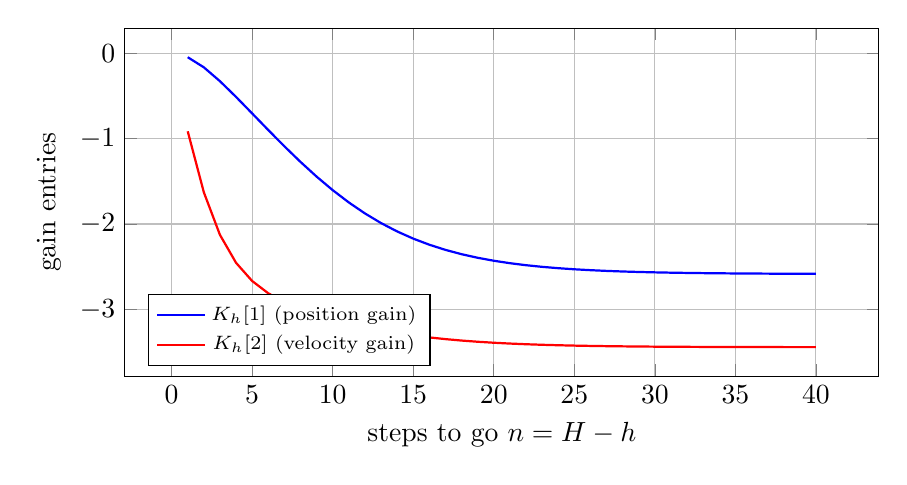
\begin{tikzpicture}
\begin{axis}[width=0.92\linewidth,height=6cm,xlabel={steps to go $n=H-h$},ylabel={gain entries},legend pos=south west,grid=both,legend style={font=\scriptsize}]
\addplot[blue,thick] coordinates {(1,-0.0454) (2,-0.1638) (3,-0.3262) (4,-0.5107) (5,-0.704) (6,-0.8985) (7,-1.0891) (8,-1.272) (9,-1.4441) (10,-1.6029) (11,-1.7469) (12,-1.8755) (13,-1.9886) (14,-2.0867) (15,-2.1709) (16,-2.2425) (17,-2.3029) (18,-2.3534) (19,-2.3954) (20,-2.4302) (21,-2.4588) (22,-2.4824) (23,-2.5016) (24,-2.5174) (25,-2.5303) (26,-2.5407) (27,-2.5492) (28,-2.5562) (29,-2.5618) (30,-2.5663) (31,-2.57) (32,-2.573) (33,-2.5754) (34,-2.5774) (35,-2.579) (36,-2.5803) (37,-2.5813) (38,-2.5821) (39,-2.5828) (40,-2.5834)};
\addlegendentry{$K_h[1]$ (position gain)}
\addplot[red,thick] coordinates {(1,-0.9134) (2,-1.6279) (3,-2.1267) (4,-2.4543) (5,-2.6676) (6,-2.8114) (7,-2.9148) (8,-2.9948) (9,-3.0605) (10,-3.1165) (11,-3.1653) (12,-3.2079) (13,-3.2451) (14,-3.2773) (15,-3.305) (16,-3.3286) (17,-3.3486) (18,-3.3654) (19,-3.3794) (20,-3.391) (21,-3.4006) (22,-3.4085) (23,-3.415) (24,-3.4203) (25,-3.4247) (26,-3.4282) (27,-3.4311) (28,-3.4334) (29,-3.4353) (30,-3.4369) (31,-3.4381) (32,-3.4391) (33,-3.4399) (34,-3.4406) (35,-3.4412) (36,-3.4416) (37,-3.4419) (38,-3.4422) (39,-3.4425) (40,-3.4426)};
\addlegendentry{$K_h[2]$ (velocity gain)}
\end{axis}
\end{tikzpicture}
\caption{Original illustration (not on the slides). Riccati iteration for a discretised double integrator, $F_x=\begin{bmatrix}1&0.1\\0&1\end{bmatrix}$, $F_u=\begin{bmatrix}0.005\\0.1\end{bmatrix}$, $C_x=I$, $C_u=0.1$, $P_H=C_x$, $H=40$. Far from the end of the episode the gains change very slowly, near the end ($n$ small) they shrink to zero: there is little time left to pay off.}
\end{figure}
\begin{figure}[H]
	\centering
	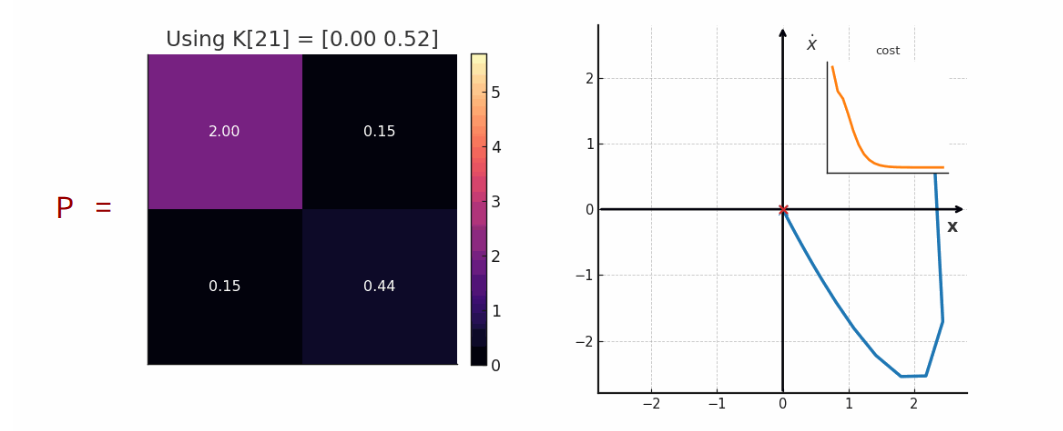
\includegraphics[width=1.0\linewidth]{1792135412968.png}
	\caption{$P[h]$ as a heat map, the current gain $K[h]$ and the state-space trajectory}\label{fig:1792135412968}
\end{figure}
\begin{intuition}
LQR is value iteration where the whole value table is replaced by a single matrix $P_h$. One backward pass of cheap matrix algebra gives the \emph{optimal controller for every time and every state}, with no grid. It is a controller, not just a plan: $u=K_hx$ tells you what to do from \emph{wherever you end up}, which makes it robust to disturbances. Note also that $K_h$ does not depend on the initial state at all.
\end{intuition}

%=====================================================================
\section{LQR Extensions \slides{71--76}}
%=====================================================================

The extensions make LQR applicable to: affine systems, systems with stochasticity, regulation around a non-zero fixed point for non-linear systems, trajectory following for non-linear systems, \dots

\subsection{LQR for Linear Time Varying (LTV) Systems \slides{72--73}}

LTV system: $x_{t+1}=F_{x,t}x_t+F_{u,t}u_t$, cost $c(x_t,u_t)=x_t^\top Q_tx_t+u_t^\top R_tu_t$ (so $F_x,F_u,C_x,C_u$ all carry the index $t$). Going backwards ($i=1,2,\dots$) the same recursion holds with time-indexed matrices:
\begin{align*}
K^*_{H-i}&=-\big(C_{u,H-i}+F_{u,H-i}^\top P_{H-i+1}F_{u,H-i}\big)^{-1}F_{u,H-i}^\top P_{H-i+1}F_{x,H-i},\\
P_{H-i}&=C_{x,H-i}+K^{*\top}_{H-i}C_{u,H-i}K^*_{H-i}+(F_{x,H-i}+F_{u,H-i}K^*_{H-i})^\top P_{H-i+1}(\cdots).
\end{align*}
\begin{intuition}
The proof of Theorem~\ref{thm:lqr} never used that the matrices were the same at every step; it only used one step at a time. So the same argument goes through with time-indexed matrices. This is the engine for trajectory following and iLQR below.
\end{intuition}

\subsection{LQR for Affine Systems \slides{74}}

Affine system $x_{t+1}=F_xx_t+F_uu_t+c$ with cost $x_t^\top C_xx_t+u_t^\top C_uu_t$. Re-define the state and transition by appending a constant coordinate, $z_t=[x_t;\,1]$:
\[
z_{t+1}=\begin{bmatrix}x_{t+1}\\1\end{bmatrix}=\begin{bmatrix}F_x&c\\0&1\end{bmatrix}\begin{bmatrix}x_t\\1\end{bmatrix}+\begin{bmatrix}F_u\\0\end{bmatrix}u_t=F_x'z_t+F_u'u_t,
\]
and the cost on $z$ is $z^\top\mathrm{diag}(C_x,0)z+u^\top C_uu$ (positive \emph{semi}-definite, which Theorem~\ref{thm:lqr} allows --- this is why the companion notes only ask $C_x\succeq0$). The resulting policy is affine in $x$: $u=K_{x,h}x+k_h$.
\begin{intuition}
The constant offset $c$ is a ``bias'' in the dynamics. By pretending the number $1$ is just another state that never changes, the bias becomes an ordinary linear term, and the linear machinery applies unchanged.
\end{intuition}

\subsection{LQR for Stochastic Systems \slides{75}}

Stochastic system $x_{t+1}=F_xx_t+F_uu_t+w_t$, $w_t\sim\mathcal N(0,\sigma^2I)$, cost as before. The optimal control policy is the \emph{same}; the cost-to-go has an extra term that depends on the variance of the system and cannot be controlled: $J^*_h=x_t^\top P_hx_t+p_h$, with base case $p_H=0$ and $p_h=\tr(\sigma^2P_{h+1})+p_{h+1}$.

\begin{proposition}[Certainty equivalence]\label{prop:ce}
The optimal gains $K_h$ are exactly those of Theorem~\ref{thm:lqr}, since the noise does not change the control law, and the value acquires an additive constant, $V^*_h(x)=x^\top P_hx+\sum_{\tau>h}\tr(P_\tau\Sigma)$.
\end{proposition}
\begin{proof}
In the induction step the only change is the expectation over $w$:
\[
\E\big[(F_xx+F_uu+w)^\top P_{h+1}(F_xx+F_uu+w)\big]=(F_xx+F_uu)^\top P_{h+1}(F_xx+F_uu)+\tr(P_{h+1}\Sigma),
\]
the cross terms vanishing because $\E[w]=0$ and $w$ is independent of $(x,u)$. The added term does not depend on $u$, so the minimiser is unchanged; it accumulates through the recursion as stated.
\end{proof}
\begin{intuition}
Zero-mean noise pushes you around but, on average, it has no preference for any direction, so the best \emph{response} to the state you see is unchanged: act as if there were no noise (``certainty equivalence''). The noise only costs you a fixed ``tax'' $\tr(P\Sigma)$ at every step that you cannot avoid. Example: with $\Sigma=\sigma^2I$ and $P_{h+1}=1.5$ in one dimension, each remaining step adds $1.5\sigma^2$ to the expected cost.
\end{intuition}

\subsection{Penalize for Change in Controls \slides{76}}

To penalise changes in the control rather than its magnitude, augment the state with the previous control, $x'_t=[x_t;\,u_{t-1}]$, and take $\Delta u_t=u_t-u_{t-1}$ as the new control:
\[
\begin{bmatrix}x_{t+1}\\u_t\end{bmatrix}=\begin{bmatrix}F_x&F_u\\0&I\end{bmatrix}\begin{bmatrix}x_t\\u_{t-1}\end{bmatrix}+\begin{bmatrix}F_u\\I\end{bmatrix}\Delta u_t,\qquad
\text{cost}=x'^\top C_x'x'+\Delta u^\top C_u'\Delta u,\ \ C_x'=\begin{bmatrix}C_x&0\\0&C_u\end{bmatrix}.
\]
(Check: $x_{t+1}=F_xx_t+F_u(u_{t-1}+\Delta u_t)=F_xx_t+F_uu_t$.)
\begin{intuition}
Real actuators cannot jump: a car cannot change its steering angle instantly without wearing the hardware and unsettling the passengers. By making ``the control I applied last time'' part of the state, the \emph{change} in control becomes the thing you choose and pay for, and you again have a standard LQR problem.
\end{intuition}

%=====================================================================
\section{LQR for Non-Linear Systems \slides{77--82}}
%=====================================================================

Non-linear system $x_{t+1}=f(x_t,u_t)$, cost $x_t^\top C_xx_t+u_t^\top C_uu_t$. We have a goal $(x^*,u^*)$ that is a fixed point, $x^*=f(x^*,u^*)$, and want to stabilise the system around it.

\textbf{Linearisation (slides 78--80).} First-order Taylor expansion around $(x^*,u^*)$:
\[
x_{t+1}\approx f(x^*,u^*)+\frac{\partial f}{\partial x}(x^*,u^*)(x_t-x^*)+\frac{\partial f}{\partial u}(x^*,u^*)(u_t-u^*).
\]
Let $z_t=x_t-x^*$ and $v_t=u_t-u^*$. Since $f(x^*,u^*)=x^*$,
\[
z_{t+1}=A\,z_t+B\,v_t,\qquad A=\frac{\partial f}{\partial x}(x^*,u^*),\ B=\frac{\partial f}{\partial u}(x^*,u^*),
\]
a linear system with cost $z^\top C_xz+v^\top C_uv$. \textbf{Solve it the usual way (slide 81):} $v_t=Kz_t\ \Rightarrow\ u_t=u^*+K(x_t-x^*)$.

\begin{figure}[H]
\centering
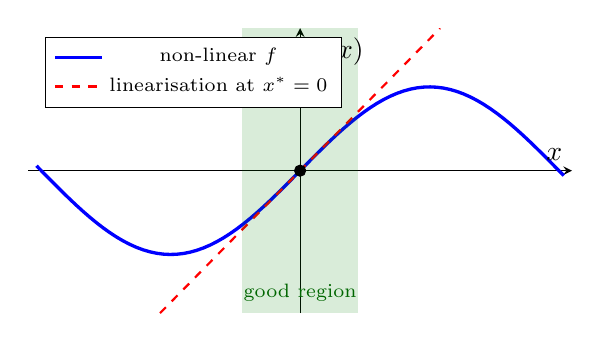
\begin{tikzpicture}
\begin{axis}[width=0.7\linewidth,height=5.2cm,xlabel={$x$},ylabel={$f(x)$},axis lines=middle,xmin=-3.3,xmax=3.3,ymin=-1.7,ymax=1.7,
  legend pos=north west,legend style={font=\scriptsize},ticks=none]
\addplot[blue,very thick,domain=-3.2:3.2,samples=80]{sin(deg(x))};
\addlegendentry{non-linear $f$}
\addplot[red,dashed,thick,domain=-1.7:1.7]{x};
\addlegendentry{linearisation at $x^*=0$}
\addplot[only marks,mark=*] coordinates {(0,0)};
\fill[green!50!black,opacity=0.15] (axis cs:-0.7,-1.7) rectangle (axis cs:0.7,1.7);
\node[green!40!black,font=\scriptsize] at (axis cs:0,-1.45) {good region};
\end{axis}
\end{tikzpicture}
\caption{Original illustration (not on slides): \textbf{Near the fixed point the tangent is a good model of $f$ (shaded), far from it it is not.}}
\end{figure}

\textbf{Linearising the cost (slide 82).} We can also linearise the cost with a 2nd-order Taylor expansion (``do it at home''), which gives something like
\[
x_t^\top C_xx_t+u_t^\top C_uu_t+u_t^\top Mx_t+x_t^\top q+u_t^\top r+c,
\]
i.e.\ a quadratic with a \emph{cross term} $M$, linear terms $q,r$ and a constant $c$. The linear terms are handled by the constant-coordinate trick, the cross term by the cross-term form of Theorem~\ref{thm:lqr}.

\begin{intuition}
Zoom in enough on any smooth curve and it looks like a straight line. LQR on the linearised system is optimal for the \emph{linear} approximation; it is a good controller as long as the state stays close to the point you linearised around --- which is what a regulator tries to do. Think of balancing a pole: you only care about small deviations from upright.
\end{intuition}

%=====================================================================
\section{LQR for Trajectory Following in Non-Linear Systems \slides{83--85}}
%=====================================================================

Non-linear system $x_{t+1}=f(x_t,u_t)$; given a trajectory $x^*_0,\dots,x^*_T$ we want controls such that $x^*_{t+1}=f(x^*_t,u^*_t)$ along the trajectory; in other words we solve (slide 84)
\[
\min_{u_0,\dots,u_{H-1}}\ \sum_{t=0}^{H-1}(x_t-x_t^*)^\top C_x(x_t-x^*_t)+(u_t-u^*_t)^\top C_u(u_t-u^*_t)\quad\text{s.t. } x_{t+1}=f(x_t,u_t).
\]
We use the same trick, but linearise around $(x^*_t,u^*_t)$ --- the linearisation point \emph{changes with $t$}, so we get an LTV system (slide 85): with $z_t=x_t-x^*_t$ and $v_t=u_t-u^*_t$,
\[
z_{t+1}\approx A_tz_t+B_tv_t,\quad A_t=\frac{\partial f}{\partial x}(x^*_t,u^*_t),\ B_t=\frac{\partial f}{\partial u}(x^*_t,u^*_t),
\]
which is solved with LQR for LTV systems, giving $u_t=u^*_t+K_t(x_t-x^*_t)$.

\begin{intuition}
Regulating around a point is the special case where the target never moves. Following a trajectory is regulating around a \emph{moving} point: at each time you linearise the world around where you \emph{should} be, and compute the gain that pulls you back onto the path. This is the idea you need for iLQR: if the trajectory you are tracking is the one you are currently trying to improve, you get a sequence of better and better LQR problems.
\end{intuition}

%=====================================================================
\section{Iterative LQR (iLQR) \slides{86--92}}
%=====================================================================

\subsection{Iterative LQR (iLQR) \slides{86}}

iLQR attempts to solve the \emph{most general case} $\min\sum_{h=0}^{H}g_h(x_h,u_h)$ subject to $x_{t+1}=f(x_t,u_t)$, by iteratively approximating it and leveraging the LQR formulation.

\subsection{Iterative LQR --- Algorithm \slides{87}}

\begin{algorithm}[Iterative LQR]\label{alg:ilqr}
\emph{Initialisation:} pick either a control policy $\pi^{(0)}$ or a sequence $\{\bar x^{(0)}_t,\bar u^{(0)}_t\}_{t=0}^H$ (by simulating any policy or by guessing). For $i=0,\dots,I$:
\begin{enumerate}[nosep]
  \item execute (or simulate) $\pi^{(i)}$ and collect $\{\bar x^{(i)}_t,\bar u^{(i)}_t\}_{t=0}^H$;
  \item obtain the LQ approximation of the problem, linearising around $\{\bar x^{(i)}_t,\bar u^{(i)}_t\}$ with a 1st-order Taylor expansion for the dynamics and a 2nd-order one for the cost, giving a time-varying linear-quadratic problem in the deviations;
  \item compute $\pi^{(i+1)}$ with the LQR-LTV formulation, in its cross-term form and augmenting the state with a constant coordinate as for affine dynamics: the expanded cost has a linear term wherever its gradient along the reference is not zero, the constant coordinate turns its part in $\delta u_t$ into a mixed term, and its Hessian may couple $\delta x_t$ and $\delta u_t$ as well. The solution is an \emph{affine} policy $\delta u_t=k^{(i)}_t+K^{(i)}_t\delta x_t$;
  \item roll the true system forward under $u_t=\bar u^{(i)}_t+k^{(i)}_t+K^{(i)}_t(x_t-\bar x^{(i)}_t)$ to obtain the next trajectory, and iterate.
\end{enumerate}
\end{algorithm}

\subsection{Iterative LQR --- LTV \slides{88--89}}

With $z_t=[x_t-\bar x^{(i)}_t;\ 1]^\top$ and $v_t=u_t-\bar u^{(i)}_t$ the dynamics are
\[
F_{x,t}=\begin{bmatrix}\frac{\partial f}{\partial x}(\bar x^{(i)}_t,\bar u^{(i)}_t)&f(\bar x^{(i)}_t,\bar u^{(i)}_t)-\bar x^{(i)}_{t+1}\\0&1\end{bmatrix},\qquad
F_{u,t}=\begin{bmatrix}\frac{\partial f}{\partial u}(\bar x^{(i)}_t,\bar u^{(i)}_t)\\0\end{bmatrix},
\]
(the top-right block is zero when the reference is a true rollout), and, assuming $g(x,u)=g(x)+g(u)$ (separable), the 2nd-order expansion of the cost $g(x_t,u_t)\approx z_t^\top C_{x,t}z_t+v_t^\top C_{u,t}v_t+2z_t^\top N_tv_t$ has
\[
C_{x,t}=\begin{bmatrix}\tfrac12\frac{\partial^2g}{\partial x^2}&\tfrac12\frac{\partial g}{\partial x}\\\tfrac12\big(\frac{\partial g}{\partial x}\big)^\top&g(x)+g(u)\end{bmatrix},\quad
C_{u,t}=\tfrac12\frac{\partial^2g}{\partial u^2},\quad
N_t=\begin{bmatrix}0\\\tfrac12\big(\frac{\partial g}{\partial u}\big)^\top\end{bmatrix},
\]
all evaluated at $(\bar x^{(i)}_t,\bar u^{(i)}_t)$. This is exactly the \emph{quadratic approximation behind iLQR}: its $2z^\top Nv$ term is the mixed term mentioned in step~3 of Algorithm~\ref{alg:ilqr}. Check: expanding, $z^\top C_xz=\tfrac12\delta x^\top g_{xx}\delta x+g_x^\top\delta x+g$, $v^\top C_uv=\tfrac12v^\top g_{uu}v$, $2z^\top Nv=g_u^\top v$, which is the second-order Taylor expansion of $g$.

\begin{figure}[H]
	\centering
	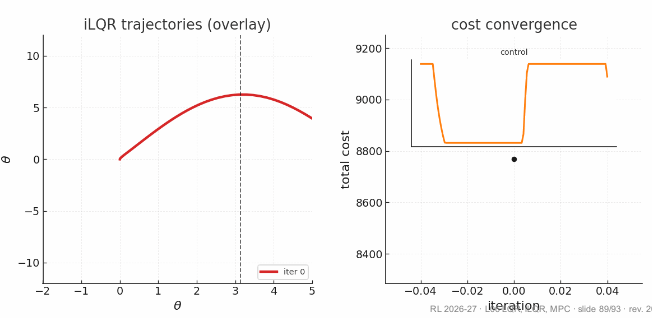
\includegraphics[width=1.0\linewidth]{1792138556885.png}
	\caption{left panel ``iLQR trajectories (overlay)'' in the $(\theta,\dot\theta)$ plane, right panel ``cost convergence''}\label{fig:1792138556885}
\end{figure}
\begin{figure}[H]
\centering
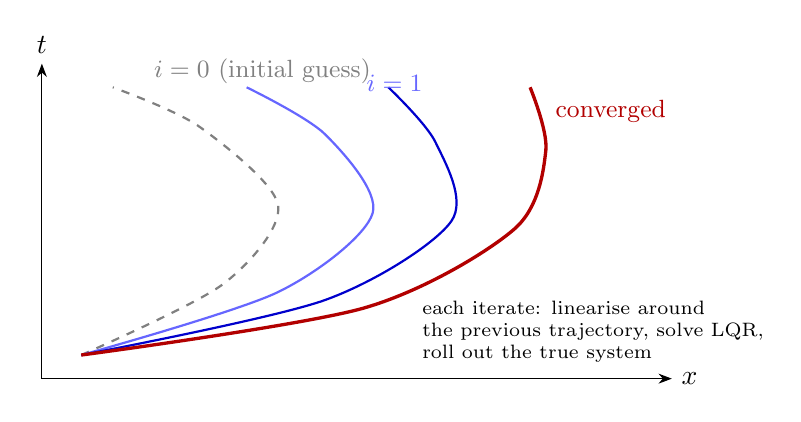
\begin{tikzpicture}[>=Stealth]
  \draw[->] (0,0)--(8,0) node[right] {$x$}; \draw[->] (0,0)--(0,4) node[above] {$t$};
  \draw[dashed,thick,gray] plot[smooth] coordinates {(0.5,0.3)(2.3,1.2)(3,2.2)(2,3.2)(0.9,3.7)};
  \draw[thick,blue!60] plot[smooth] coordinates {(0.5,0.3)(3.0,1.1)(4.2,2.1)(3.6,3.1)(2.6,3.7)};
  \draw[thick,blue!80!black] plot[smooth] coordinates {(0.5,0.3)(3.6,1.0)(5.2,2.0)(5.0,3.0)(4.4,3.7)};
  \draw[very thick,red!70!black] plot[smooth] coordinates {(0.5,0.3)(4.1,0.9)(6.0,1.9)(6.4,2.9)(6.2,3.7)};
  \node[gray,right] at (1.3,3.9) {\small $i=0$ (initial guess)};
  \node[blue!60,right] at (4.0,3.75) {\small $i=1$};
  \node[red!70!black,right] at (6.4,3.4) {\small converged};
  \node[font=\scriptsize,align=left] at (7,0.6) {each iterate: linearise around\\the previous trajectory, solve LQR,\\roll out the true system};
\end{tikzpicture}
\caption{Original schematic (not on the slides) of iLQR: each iteration replaces the nominal trajectory with the roll-out of the LQR policy of the local LQ model.}
\end{figure}

\begin{intuition}
iLQR is Newton-like optimisation done by dynamic programming. At each iteration you build a \emph{local} linear-quadratic model of the world around your current best trajectory, solve it exactly with LQR, and apply the result to the real system to get a new (better) trajectory. The affine policy $\delta u=k+K\delta x$ has two parts: $k$ is the feed-forward correction to the plan, $K$ is the feedback that keeps you on it.
\end{intuition}

\subsection{Iterative LQR --- Convergence \slides{90--91}}

As it is, iLQR might not converge: the optimal policy of the LQ approximation might end up \emph{not staying close} to the linearisation points. \textbf{Solution:} change the cost to
\[
(1-\alpha)\,g(x_t,u_t)+\alpha\big(\|x_t-\bar x^{(i)}_t\|_2^2+\|u_t-\bar u^{(i)}_t\|_2^2\big),
\]
and if $g$ is bounded and $\alpha$ is close enough to $1$, the second term dominates and ensures the linearisations are good approximations of the solution trajectory.

\begin{intuition}
It is a leash. The LQ model is only trustworthy near the nominal trajectory, so you add a penalty for straying from it. With $\alpha=0.9$, one unit of deviation costs $0.9$ while a unit of true cost counts $0.1$: the update becomes timid but safe, and you take many small, reliable steps instead of one big wrong leap. This is the same idea as a trust region.
\end{intuition}

\subsection{Iterative LQR --- Tricks \slides{92}}

\begin{itemize}[nosep]
  \item \textbf{Initialisation matters}: you can get stuck in local optima. Alternatives: simulated annealing (if there are no computation constraints) or line search.
  \item If $g$ is non-convex, the LQ approximation may give non positive-definite $C_x,C_u$. \textbf{Fix:} add more cost for deviating from the linearisation points until they become positive-definite.
\end{itemize}

%=====================================================================
\section{Receding Horizon Control, i.e.\ Model Predictive Control (MPC) \slides{93}}
%=====================================================================

At iLQR convergence, the system could execute the policy and still not be at the expected trajectory (inaccurate dynamics, noise, \dots). \textbf{Idea:} at every time step $t$ replan from $t$ to $H$. \textbf{In practice:} replanning until $H$ at every step is too costly, so replan over a \emph{shorter horizon} $h$ and use a cost-to-go $J(t+h)$ at its end. This is a Model Predictive Controller with an iLQR solver.

\begin{algorithm}[Receding-horizon control (MPC)]\label{alg:mpc}
At each time $t$: solve the control problem from the current \emph{measured} state over a short horizon $[t,t+h]$, with a terminal cost approximating the cost-to-go beyond $h$; apply only $u_t$; discard the rest; measure; repeat.
\end{algorithm}

\begin{figure}[H]
\centering
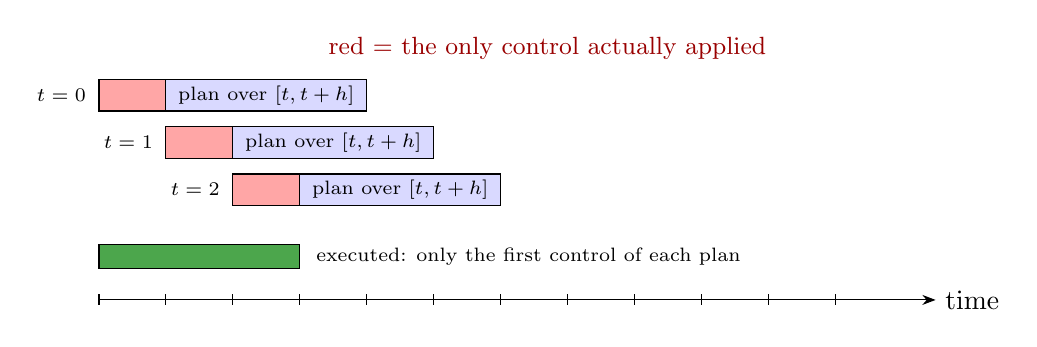
\begin{tikzpicture}[>=Stealth,xscale=0.85]
  \draw[->] (0,0)--(12.5,0) node[right] {time};
  \foreach \t in {0,1,2,3,4,5,6,7,8,9,10,11} \draw (\t,0.07)--(\t,-0.07);
  \foreach \k/\y in {0/2.4,1/1.8,2/1.2} {
    \draw[fill=blue!15] (\k,\y) rectangle (\k+4,\y+0.4);
    \draw[fill=red!35] (\k,\y) rectangle (\k+1,\y+0.4);
    \node[font=\scriptsize] at (\k+2.5,\y+0.2) {plan over $[t,t+h]$};
    \node[font=\scriptsize,left] at (\k-0.05,\y+0.2) {$t=\k$};
  }
  \draw[fill=green!50!black!70] (0,0.4) rectangle (3,0.7);
  \node[font=\scriptsize,right] at (3.1,0.55) {executed: only the first control of each plan};
  \node[font=\small,red!60!black] at (6.7,3.2) {red = the only control actually applied};
\end{tikzpicture}
\caption{Original schematic (not on the slides): the planning window slides forward at every step.}
\end{figure}

\begin{intuition}
It is the way you navigate with GPS: you do not drive the original route blindly, you recompute from where you \emph{are} after every turn. Replanning gives feedback through the optimiser, so errors due to noise or a wrong model are corrected at the next step. The finite window keeps the computation affordable, and the terminal cost-to-go $J(t+h)$ stops the controller from being short-sighted.
\end{intuition}

%=====================================================================
\section{Summary}
%=====================================================================

\subsection{Comparison of the methods}

\begin{table}[h]
\centering
\small
\renewcommand{\arraystretch}{1.25}
\begin{tabular}{@{}p{2.6cm}p{2.7cm}p{2.5cm}p{3.1cm}p{3.1cm}@{}}
\toprule
\textbf{Method} & \textbf{Setting} & \textbf{Output} & \textbf{Cost / scaling} & \textbf{Main limitation}\\
\midrule
Backward induction (Thm.~\ref{thm:bi}) & finite-horizon MDP, discrete $S,A$ & $V^*_h,\pi^*_h$ (tables), exact & $O(H|S|^2|A|)$; with a grid $\Theta((1/\epsilon)^{2d+k})$ & curse of dimensionality: only $d\lesssim5$--$6$\\
LQR (Thm.~\ref{thm:lqr}) & linear dynamics, quadratic cost & $K_h,P_h$, optimal linear feedback, exact & closed-form Riccati recursion, polynomial in $d,k$ (matrix products/inverse) & needs linear model and quadratic cost\\
LQR extensions & LTV, affine, stochastic (Prop.~\ref{prop:ce}), $\Delta u$ penalty & same recursion on augmented/time-indexed matrices & same as LQR & still linear-quadratic\\
Linearised LQR & non-linear $f$ near a fixed point or a reference trajectory & $u=u^*+K(x-x^*)$ & LQR-LTV along reference & valid only near the reference\\
iLQR (Alg.~\ref{alg:ilqr}) & general non-linear $f$, general $g$ & locally optimal affine policy / trajectory & $I\times$ (linearise + LQR-LTV) & may diverge; local optima; needs trust-region/penalty\\
MPC (Alg.~\ref{alg:mpc}) & any of the above, online & $u_t$ re-computed at every step & one short-horizon solve per step & model error, compute budget per step; needs terminal cost\\
\bottomrule
\end{tabular}
\caption{Summary of the methods of lecture L06.}
\end{table}

\begin{figure}[H]
\centering
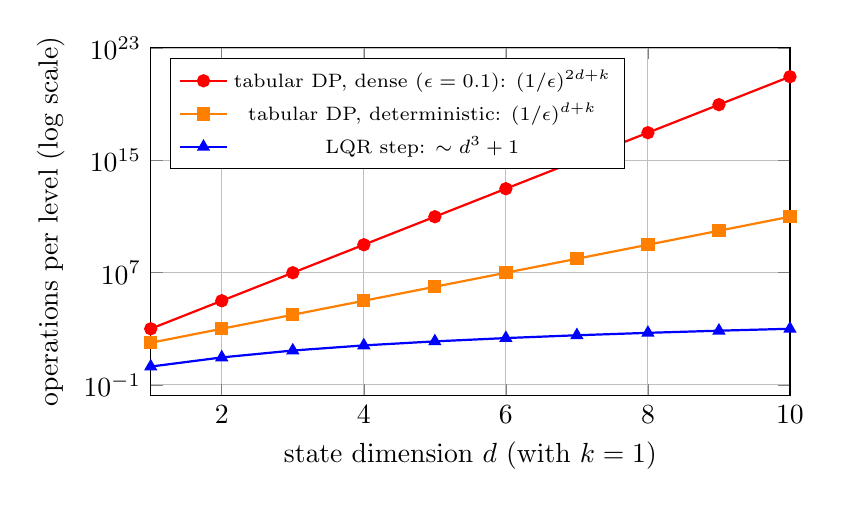
\begin{tikzpicture}
\begin{axis}[width=0.8\linewidth,height=6cm,ymode=log,xlabel={state dimension $d$ (with $k=1$)},ylabel={operations per level (log scale)},
  grid=both,legend pos=north west,legend style={font=\scriptsize},xmin=1,xmax=10]
\addplot[red,thick,mark=*] coordinates {(1,1e3)(2,1e5)(3,1e7)(4,1e9)(5,1e11)(6,1e13)(7,1e15)(8,1e17)(9,1e19)(10,1e21)};
\addlegendentry{tabular DP, dense ($\epsilon=0.1$): $(1/\epsilon)^{2d+k}$}
\addplot[orange,thick,mark=square*] coordinates {(1,100)(2,1e3)(3,1e4)(4,1e5)(5,1e6)(6,1e7)(7,1e8)(8,1e9)(9,1e10)(10,1e11)};
\addlegendentry{tabular DP, deterministic: $(1/\epsilon)^{d+k}$}
\addplot[blue,thick,mark=triangle*] coordinates {(1,2)(2,9)(3,28)(4,65)(5,126)(6,217)(7,344)(8,513)(9,730)(10,1001)};
\addlegendentry{LQR step: $\sim d^3+1$}
\end{axis}
\end{tikzpicture}
\caption{Qualitative comparison (original, order-of-magnitude, constants ignored): tabular DP grows exponentially in $d$, a Riccati step grows like a polynomial. LQR escapes the curse of dimensionality by \emph{structure} (linear dynamics, quadratic cost), not by approximation.}
\end{figure}

\subsection{Key take-aways}

\begin{itemize}
  \item \textbf{Finite horizon makes DP exact and one-pass}: backward induction from the deadline gives time-dependent optimal policies, but its cost explodes with dimension when the state is discretised (Bellman's curse).
  \item \textbf{LQR is value iteration in closed form}: for linear dynamics and quadratic cost the value is $x^\top P_hx$ and the policy is the linear feedback $u=K_hx$, computed by the Riccati recursion with no discretisation.
  \item \textbf{Extensions reduce to the same recursion}: affine terms (constant coordinate), LTV matrices, penalties on $\Delta u$ (augmented state); additive zero-mean noise leaves the gains unchanged (certainty equivalence) and only adds $\tr(P\Sigma)$ to the cost.
  \item \textbf{Non-linear problems are handled by repeated local LQR}: linearise around a point or a trajectory (regulation, tracking), and iterate in iLQR with 1st-order dynamics and 2nd-order cost; keep the iterates close to the linearisation points (penalty weight $\alpha$) and watch for local optima and non positive-definite Hessians.
  \item \textbf{MPC adds feedback through replanning}: solve over a short horizon from the measured state, apply the first control only, repeat; this makes the system robust to model error and noise at the price of one solve per time step.
\end{itemize}

%=====================================================================
\appendix
\section{Supplementary material (in the companion PDFs, not on the slides)}\label{app:supp}
%=====================================================================

The following result is in the companion notes ``Finite-horizon MDPs and optimal control'' but has \textbf{no corresponding slide}: the slides only state (slides 13--15) that policies are time-dependent, without an example proving it is necessary.

\begin{proposition}[The optimal policy depends on the time remaining]\label{prop:timedep}
There are finite-horizon MDPs in which every optimal policy satisfies $\pi^*_h(s)\ne\pi^*_{h'}(s)$ for some state $s$ and some $h\ne h'$.
\end{proposition}
\begin{proof}
Two actions at a single state $s$. Action \emph{safe} pays $1$ and returns to $s$. Action \emph{gamble} pays $0$ now and moves to an absorbing state $g$ paying $3$ per step with probability $1/2$, or to an absorbing state $b$ paying $0$ per step with probability $1/2$. Write $n=H-h$ for the number of steps remaining and $V_n$ for the optimal value at $s$ with $n$ steps left, $V_0=0$. Gambling now is worth $Q_n(\text{gamble})=\tfrac12\cdot3(n-1)=1.5(n-1)$, since the first step pays nothing and the remaining $n-1$ pay $3$ half the time; playing safe now is worth $Q_n(\text{safe})=1+V_{n-1}$, one now and the best play afterwards.

For $n\le3$ safe is optimal throughout: by induction $V_{n-1}=n-1$, so $Q_n(\text{safe})=n$, which beats $1.5(n-1)$ at $n\le2$ and ties with it at $n=3$, giving $V_3=3=1.5\cdot2$. From there $V_{n-1}=1.5(n-2)$ by induction, and
\[
Q_n(\text{gamble})-Q_n(\text{safe})=1.5(n-1)-1-1.5(n-2)=\tfrac12>0\qquad(n\ge4),
\]
so the gamble is optimal and $V_n=1.5(n-1)$, which carries the induction. So safe is strictly better for $n\le2$, the two tie at $n=3$, and the gamble is strictly better for $n\ge4$. Any optimal policy therefore gambles early in a long episode and plays safe in the last two steps.
\end{proof}

\begin{figure}[H]
\centering
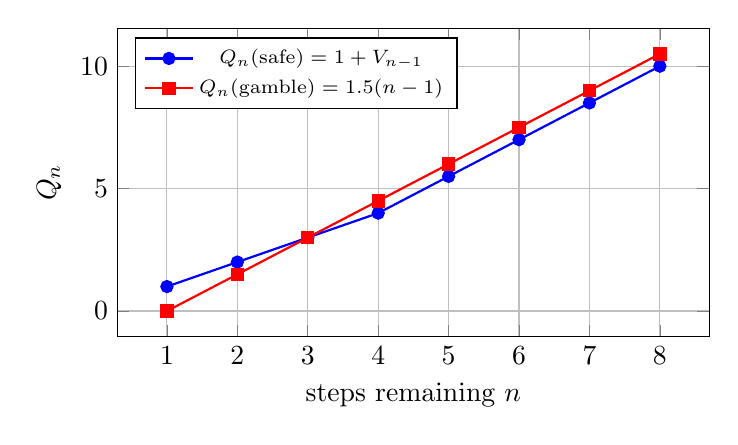
\begin{tikzpicture}
\begin{axis}[width=0.75\linewidth,height=5.5cm,xlabel={steps remaining $n$},ylabel={$Q_n$},xtick={1,...,8},legend pos=north west,grid=both,legend style={font=\scriptsize}]
\addplot[blue,thick,mark=*] coordinates {(1,1)(2,2)(3,3)(4,4)(5,5.5)(6,7)(7,8.5)(8,10)};
\addlegendentry{$Q_n(\text{safe})=1+V_{n-1}$}
\addplot[red,thick,mark=square*] coordinates {(1,0)(2,1.5)(3,3)(4,4.5)(5,6)(6,7.5)(7,9)(8,10.5)};
\addlegendentry{$Q_n(\text{gamble})=1.5(n-1)$}
\end{axis}
\end{tikzpicture}
\caption{Values of the two actions in the proof of Proposition~\ref{prop:timedep} (original figure). The curves cross at $n=3$.}
\end{figure}

\begin{intuition}
Gambling pays off only if there is enough time to harvest the jackpot: the expected gain per remaining step ($1.5$) beats the safe payoff ($1$) only if enough steps remain to compensate for the one step you give up. Concretely, with $n=2$ you get $2$ safe versus $1.5$ from gambling, with $n=4$ you get $4$ versus $4.5$. The identical state calls for different actions at different times, so no single stationary policy can be optimal; this justifies the time-dependent policies $\pi=(\pi_0,\dots,\pi_{H-1})$ of Definition~\ref{def:fhmdp}.
\end{intuition}

\paragraph{A note on the companion notes' ``slides only'' items.} The self-check of the LQR PDF lists as ``on the slides only'' the derivations for affine dynamics, penalising changes in control, LQR around a fixed point, trajectory following, and the quadratic approximation behind iLQR. They are in the main text at their slide position (Sections on LQR Extensions, Non-Linear Systems, Trajectory Following, iLQR).

\end{document}